\chapter{索引づけ}
\ref{chap:er-model}章や\ref{chap:normalization}章で説明した実体関連モデルと正規化理論によって，データを正しく矛盾なく管理するための関係データベースを設計することができるようになりました．
しかし，データの正しさをガチガチに担保できるようになっても，問い合わせにかかる待ち時間が長いようではデータベースとして使い物になりません．
利便性が高いデータベースには，データの管理のしやすさに加え，データの処理速度も求められます．

ところで，これまでの章で見てきたように，関係データベースに格納されたデータは，複数のテーブルに分割されていることがほとんどです．
そのため，必要なデータを取得するには，
\begin{itemize}
\item 関係する複数のテーブルを結合し
\item 結合したテーブルのレコードから条件に合致するものを抽出する
\end{itemize}
といった処理が必要となります．
さて，テーブルの結合は，結合元のテーブルの各レコードに対し，結合先のテーブルから条件に合致するレコードを検索してつなぎ合わせる処理であることを思い出してください．
ということは，結合元と結合先のテーブルのレコード数が多いほど，処理が重くなりそうです．
例えば，結合元と結合先のテーブルのレコード数がそれぞれ100万件ある場合，レコードのすべての組み合わせについて条件を満たすかを逐一チェックすると，合計1兆ペアも確認しなければなりません．
確認回数が多いと，それに比例してテーブルの結合にかかる時間は長くなってしまいます．

この問題を解決する技術が\strong{索引づけ（indexing）}です\footnote{データベースの応答速度（クエリ実行時間）を改善する方法としては，索引づけ以外にもクエリ最適化（query optimization）などがあります}．
索引づけを行うことで，データベースは条件に合致するレコードの検索速度を大幅に改善することができます．
本章では，索引づけの基本的な考え方と，索引づけに使われる代表的なデータ構造であるB+木とハッシュ索引について説明します．


\section{関係データの物理的な格納方法}
計算機ではあらゆるデータはゼロイチの2進数で表現され，主記憶装置（メモリ）やハードディスクやSSDのような補助記憶装置のどこかに物理的に格納されています．
このことは，計算機を使う関係データベースにおいても同じです．
関係データベースではすべてのデータはテーブルとして表現されますが，データを補助記憶装置に格納する際，テーブルを構成する複数のレコードはひとまとまりの単位（ブロック）に分割され，記憶装置のどこかに格納されます．

% \begin{notebox}
% 表データをタプル（レコード）単位で分割し格納するデータベースは\strong{行指向データベース（row-oriented database）}と呼ばれます．
% それに対して，属性（列）単位で分割・格納するデータベースは\strong{列指向データベース（column-oriented database）}と呼ばれます．

% 関係データベースのようにレコードの追加や削除を頻繁に行うことが想定されるデータベースにおいては，行指向でデータを格納するほうが効率的です．
% 一方，データの更新が頻繁でなく，属性（列）単位の集約演算を頻繁に行うような場合は，列指向データベースの方が効率的です．
% \end{notebox}

図\ref{fig:data-store}は，「商品」テーブルを（物理的な）記憶媒体に格納する際のイメージ図です．
図のように，「商品」の各レコードは記憶装置の特定の場所にばらばらに格納されます．
SQL文による問い合わせが行われると，関係データベースシステムは条件に合致するレコードが記憶装置のどの場所に保存されているか（アドレス）を調べ，該当する場所から具体的なデータを取得します．

\begin{figure}[tb]
    \centering
    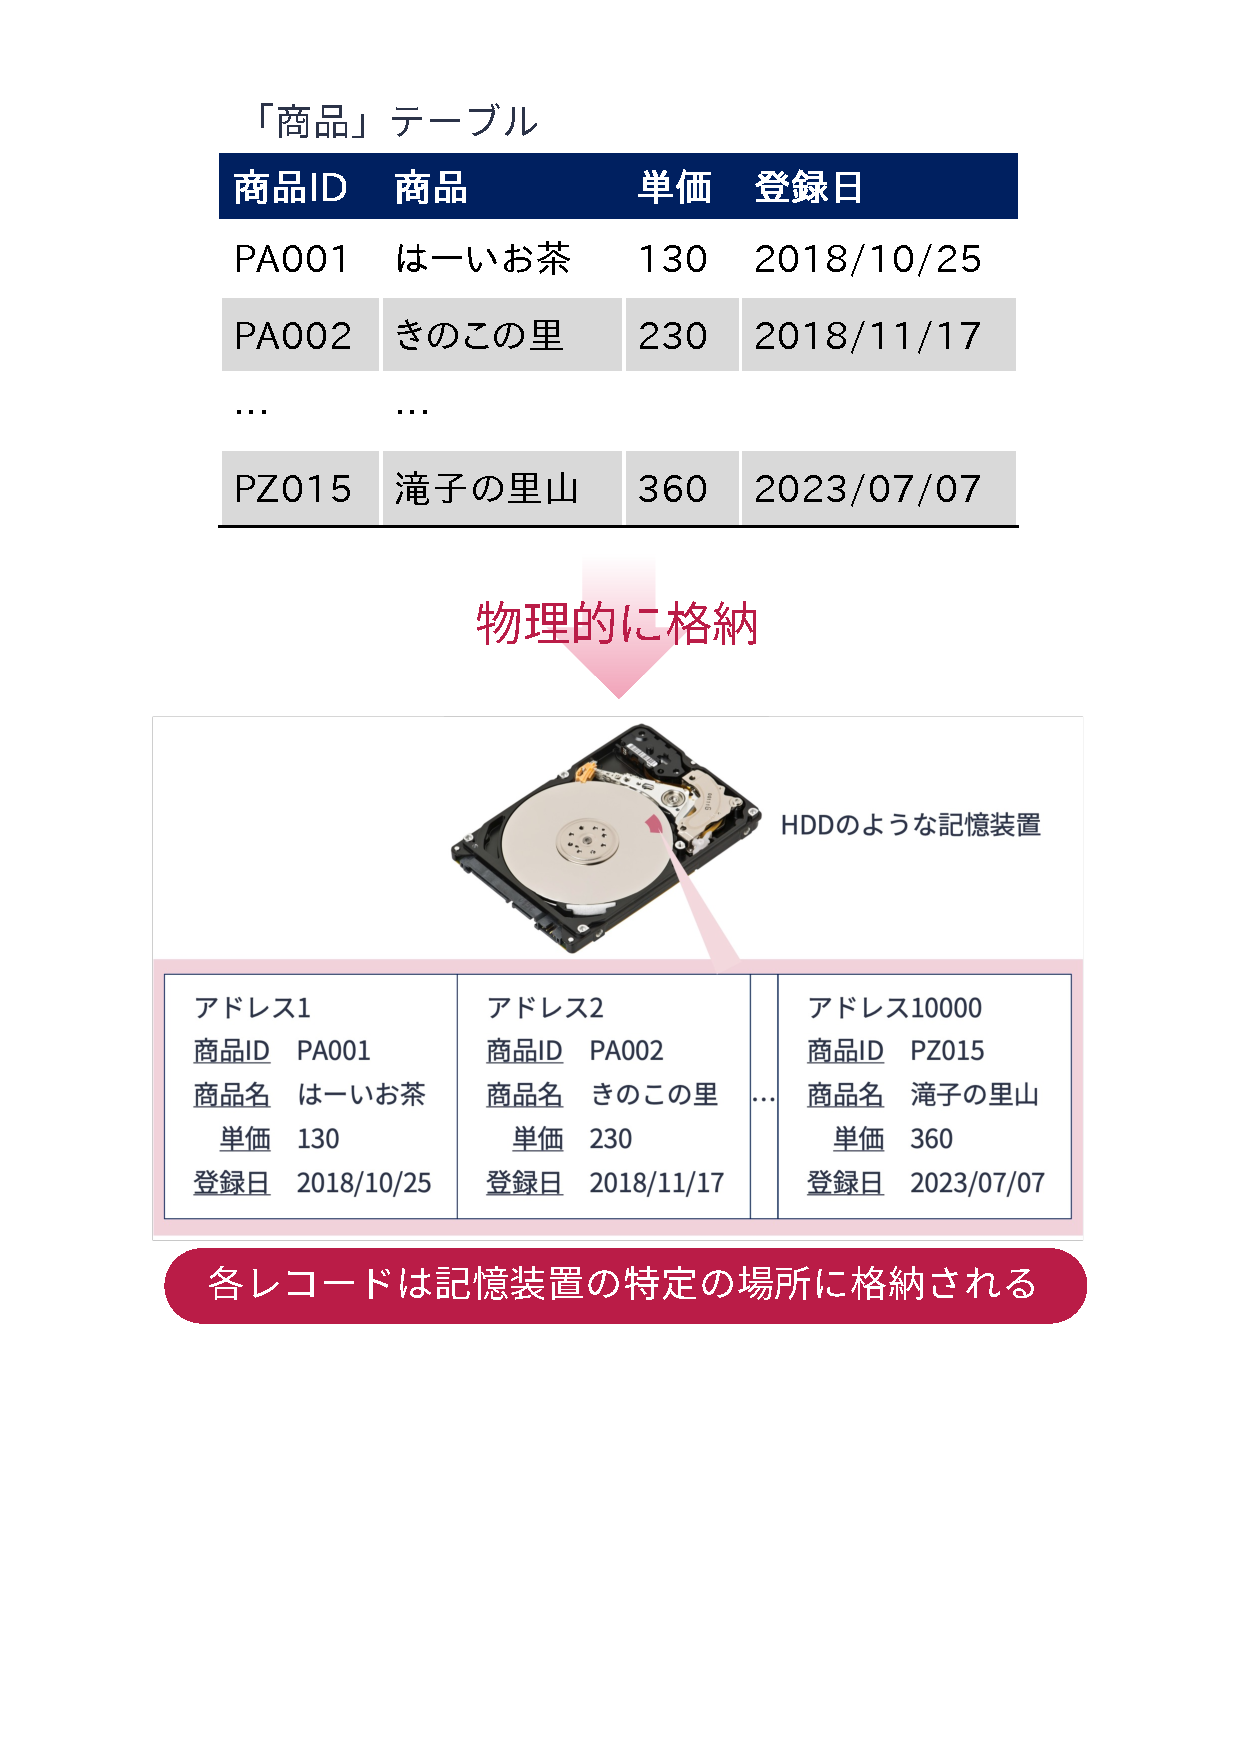
\includegraphics[width=0.8\textwidth]{figure/indexing/data-store.pdf}
    \caption{関係データの物理的な格納方法のイメージ}
    \label{fig:data-store}
\end{figure}


\section{索引}
データベースから条件に合致するレコードを探す方法として，該当するテーブルのレコードが格納されている場所を先頭から1つ1つ調べ上げる方法が考えられます．
この方法では，レコードの数が$N$件ある場合，$N$回確認作業が必要となります．
問い合わせへの応答時間は，確認回数に比例して長くなります．
レコードの数が少ない，つまり$N$が小さい場合は問題となりません．
しかし，ビジネスの現場等で用いられる関係データベースは，膨大な数のレコードを扱います．
計算が得意な計算機とはいえ，数百万，数千万のレコード数を逐次的にチェックするにはそれなりに時間がかかります．

\strong{索引づけ（indexing）}は，レコードの探索時間を改善したいときに有効な方法の1つです．
一般に索引といえば，書籍の末尾に掲載された，特定の項目が書籍中のどのページに掲載されているかをまとめ，項目順に並べたものを思い浮かべます．
書籍の場合，図\ref{fig:book-index}のように索引を調べることで，全ページを見返さなくても自分が知りたい項目がどこのページに掲載されているかをカンタンに知ることができます．
\begin{figure}[tb]
    \centering
    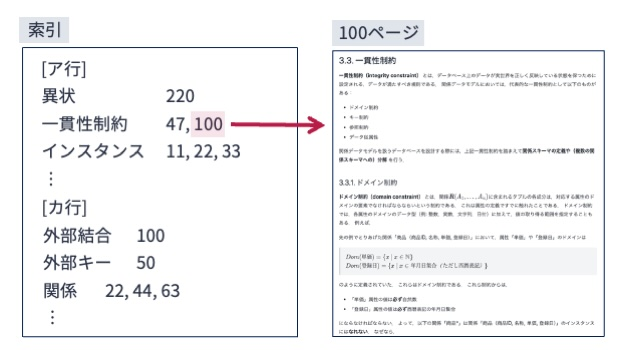
\includegraphics[width=1.0\textwidth]{figure/indexing/book-index.jpg}
    \caption{書籍における索引の例}
    \label{fig:book-index}
\end{figure}

データベースにおける索引も書籍のそれと類似した役割をもちます．
データベースにおける\strong{索引（インデックス; index）}とは，データベース中のある属性に注目し，ある属性値を持つレコードを効率よく取得できるよう工夫された特殊なデータです．
索引は
\begin{itemize}
\item \strong{索引キー（index key）}と呼ばれる検索対象となる属性の値，および
\item その値をもつレコードの場所を特定する情報（記憶装置の中でレコードが格納されている場所）
\end{itemize}
から構成されます．

図\ref{fig:db-index}は「商品」テーブルの属性「単価」に関する索引，およびそれを利用した問い合わせのイメージです．
「単価」の索引には，単価の値（索引キー）とその値をもつレコードが格納された場所のペアが記載されています．
この索引を使えば，ある属性値をもつレコードが格納されている場所をすぐに知ることができるため，条件に合致するレコードを効率よく取得することができます．
例えば，単価の値が\graybox{230}のレコードを検索したい場合を考えましょう．
まずは索引を上から調べていき，\graybox{230}の値がどこにあるかを調べます．
図の例では，\graybox{230}の値を持つレコードの場所は\graybox{2}であることが分かります．
場所が分かれば，指定された記憶装置の場所（アドレス\graybox{2}）を調べに行くことで欲しいレコードの情報を得ることができます．
\begin{figure}[tb]
    \centering
    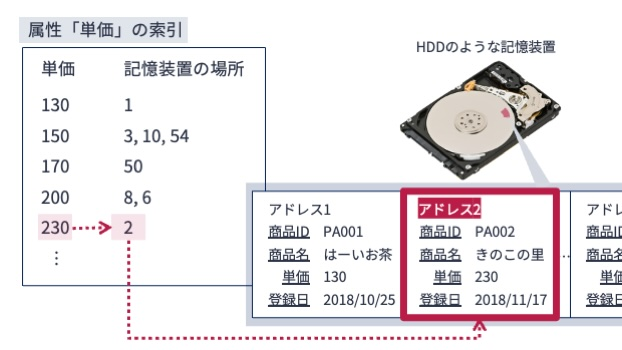
\includegraphics[width=1.0\textwidth]{figure/indexing/db-index.jpg}
    \caption{データベースにおける索引の例}
    \label{fig:db-index}
\end{figure}

書籍における索引は「わざわざ」本の末尾に索引用ページ（場所）を作っています．
それと同様，データベースの索引についても「わざわざ」記憶装置の場所（空間）を消費して索引用データを作っています．
索引は\strong{空間効率を犠牲にして時間効率を向上させる方法}です．
空間効率の劣化を抑えつつ時間効率を向上させるために，様々な種類の索引が提案されています．


\section{二分探索}
例えば，格納されたレコード数が10万のテーブルに対して，ある属性に関する索引を構築したとしましょう．
索引のサイズ（索引キーの数）が索引付けの対象となるレコード数の5分の1になった場合，索引リストの先頭から索引キーの値を一つ一つ調べていく線形探索を行うと，最悪2万回もの確認が必要となります．
索引を使えば，特定の条件を満たすレコードが探しやすくなる -- 直感的にはその通りなのですが，索引（キーのリスト）も巨大になってしまうと，そこから条件に合致する箇所を探すのにも効率の良い方法が必要となります．

索引キーがソートされている場合には，索引の探索効率を劇的に向上させる方法として二分探索が使えます．
\strong{二分探索（binary search）}は，ソート済みの配列から指定した値を高速に探索するアルゴリズムです．
二分探索アルゴリズムの概要は以下の通りです：
\begin{enumerate}
\item 配列のちょうど真ん中の位置の値をチェックする．チェックした値が探している値の場合，そこで終了
\item チェックした値が探している値よりも
    \begin{itemize}
    \item 「小さかった」場合，配列の「右半分」を新たな検索対象配列とする
    \item 「大きかった」場合，配列の「左半分」を新たな検索対象配列とする
    \end{itemize}
\item 値が見つかるまで，ステップ1-2を繰り返す．配列の長さが1になっても見つからなかったら，探している値は配列にはなかったことになる
\end{enumerate}

図\ref{fig:binary-search}を使って，二分探索の振る舞いを確認してみましょう．
図の一番上には，ソートされた索引キーの配列が並んでいます．
配列の位置は索引における行番号と考えてください．
今，\graybox{270}という値（をもつレコード）の場所がどこかを知りたいとしましょう．
配列の先頭から愚直に調べていくと，\graybox{270}の値が入った場所を見つけるには計5回の確認が必要となります．

一方，二分探索を適用すると，以下のような手順で値の場所が見つかります．
\begin{figure}[tb]
    \centering
    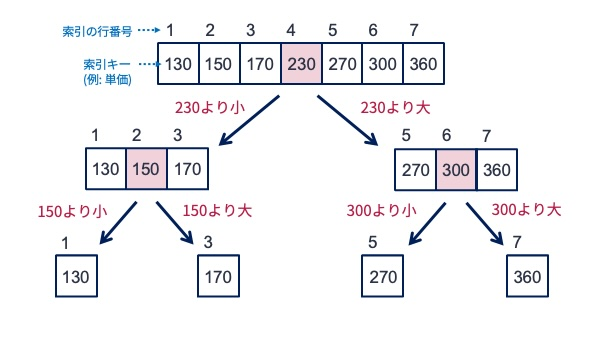
\includegraphics[width=1.0\textwidth]{figure/indexing/binary-search.jpg}
    \caption{二分探索のイメージ}
    \label{fig:binary-search}
\end{figure}
\begin{enumerate}
\item まず配列の真ん中である4番目にアクセスし値を見る（値=\graybox{230}）
\item 所望の値である\graybox{270}は\graybox{230}より大きいので，右半分の配列の真ん中の位置（6番目）にアクセスする（値=\graybox{300}）
\item 所望の値である\graybox{270}は\graybox{300}より小さいので，先ほど確認した配列の左半分の真ん中（5番目しかない）にアクセスする
\item 値が\graybox{270}であったので，位置情報として\graybox{5}を返す（終了して，索引の5行目に記されている記憶装置の場所にあるレコードを調べに行く）
\end{enumerate}

\graybox{270}の値を見つけるのに要した配列へのアクセス回数は合計3回となります．
二分探索では，1ステップごとに調査対象となる配列のサイズが半分になります．
そのため，もとの配列のサイズが$N$のとき，所望の値を見つけるために必要となる配列へのアクセス回数は最悪のケースでも$\log_2 N$回となります．
図\ref{fig:binary-search}の例では配列のサイズが小さいため二分探索の効果が感じにくいですが，配列のサイズが巨大になると二分探索の効果が実感できます．
例えば索引のサイズ（索引キーの種類数）が100万の場合，二分探索を使えば索引キーの配列に20回（$\log_2 10^6$回）程度アクセスするだけで所望の値を見つけることができます．


\section{B+木}
二分探索はソート済み配列を探索する上で強力な方法ですが，データベースの索引キーの探索に使うには以下のような欠点があります．
\begin{itemize}
\item データベースが超巨大になると索引のサイズも超巨大になるため，さすがの二分探索も遅くなる\footnote{索引データが大きすぎると高速なメモリに収まりきらないため，動作の遅いディスク（補助記憶装置）に配置することになります．二分探索はデータ全体をあちこち飛び飛びに確認しますが，ディスクのような補助記憶装置では読み取り操作が遅く，そのような操作が何度も発生してしまうと，それが検索スピードの足かせとなってしまいます．}
\item 属性値がある範囲の値をもつレコードを探索したいというケースにおいて，単一の値の検索に特化した二分探索は分が悪い
\item データベースではレコードの追加や更新が頻繁に発生するため，データベースの更新ごとに巨大な索引キーをソートするのは効率が悪い（定番のソートアルゴリズム「クイックソート」を使っても$O(N \log N)$の計算時間がかかる）
\end{itemize}

\strong{B+木（B+ tree）}\footnote{諸説ありますが，データベースの教科書として著名な``Principles of Database Systems (Jeffrey Ullman著)''によると，B+木の``B''はbalancedの頭文字に由来しています．}は，二分探索よりも高速かつ効率よくデータの探索を行え，かつ更新にかかるコストも小さい，データベース索引用のデータ構造です\cite{Knuth本}．
索引のリストが巨大になっても高速に探索できるよう，B+木は索引を階層的に管理することで，二分探索の欠点を克服しています．
B+木は以下のような特徴を持つ木構造データです（$d$および$e$の値は事前に決めておく）．
\begin{enumerate}
\item 根ノードから葉ノードへのパスの長さはすべて同じである
\item 葉ノードは索引キーの（順序付き）集合で構成される．各葉ノードは索引キーを収容するスペースをもつ．そのスペースには最小$\lceil \frac{e}{2} \rceil$個，最大$e$個の索引キーを収容できる．なお，葉ノード中の索引キーは昇順にソートされている
\item 隣接する葉ノードはリンクで結ばれている（すぐ隣の索引キーが何か分かる）
\item 葉ノード以外のノードは，ポインタと探索キーを交互に持つ．なお，ノードに収容できるポインタの数は最大で$2d+1$個，探索キーは最大$2d$個である．探索キー$k$の左隣のポインタは値が$k$未満の探索キーを含む子ノードにリンクしている．探索キー$k$の右隣のポインタは値が$k$以上の探索キーを含む子ノードにリンクしている
\item 根ノードは1個以上の探索キーを持つ
\item 根ノード，葉ノード以外の中間ノードは$d$個以上の探索キーを持つ
\item 葉ノードの各索引キーはその値を属性値としてもつレコード集合とリンクしている（記憶装置で該当レコードが記録されている位置にすぐ飛べる）
\end{enumerate}
なお，$d$の値をB+木の\strong{次数}と呼びます．

上の定義だけでは分かりづらいので，図\ref{fig:b+tree}を見ながらB+木の特徴を確認しましょう．
ある属性$A$の索引キー（属性値）として
\begin{equation*}
1, 4, 9, 16, 25, 36, 49, 64, 81, 100, 121, 144,169, 196, 225, 256
\end{equation*}
のいずれかを取るレコードを格納したテーブルがあるとします．
図\ref{fig:b+tree}は，このテーブルの属性$A$に関するB+木です．
なお，このB+木は$d=1，e=3$としています．
\begin{figure}[tb]
    \centering
    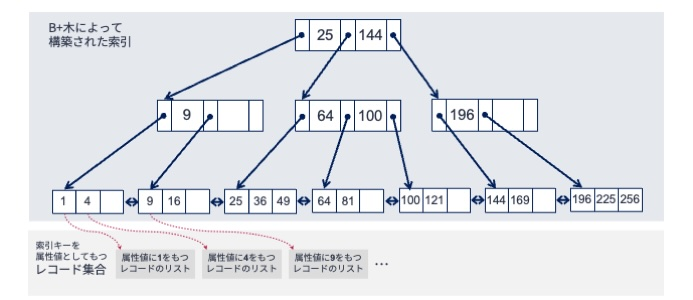
\includegraphics[width=1.0\textwidth]{figure/indexing/b+tree.jpg}
    \caption{属性$A$に関するB+木の例（$d=1, e=3$）}
    \label{fig:b+tree}
\end{figure}

図を見たら分かるように，すべての索引キーはいずれかの葉ノードに格納されています（特徴2）．
索引キーが格納されたどの葉ノードについても，根ノードから2回枝をたどるだけで到達できます（特徴1）．
また，根以外のどのノードも半数以上スペースが埋まっています（特徴2および6）．
さらに，ある索引キーの次に小さい（大きい）索引キーは同じ葉ノード内で隣接している，もしくは隣接する葉ノード内に存在しています（特徴3）．
そのため，例えば索引キーの\graybox{4}の次に大きい索引キーを知りたければ，\graybox{4}が含まれる一番左の葉ノードから右隣にリンクされている葉ノードを見ることで，\graybox{9}が次に大きい索引キーであることが分かります．

B+木において，葉ノードは，各レコードの格納場所情報を保持しているため，いわゆる索引と見なすことができます．
一方，葉ノードの親ノードは，葉ノードを振り分け，葉ノードの場所を管理しているという意味では，\strong{索引の索引}になっていると見なせます．
このように，B+木は索引を階層的に管理します．


B+木で重要なことは，どの葉ノードも\strong{根ノードからの距離が同じ}であることです．
この設計によって，どの索引キーも同じ計算時間で見つけることができます．
一方，どのノードも常に\strong{半数以上}スペースが埋まっているという特徴は，裏を返せば半分は空いていてもよいということになります．
これは索引に割り当てる記憶領域が無駄になっていると言えますが，空きがあれば木の構造を大きく変えずに新たな索引キーが挿入できるため，索引更新に柔軟性を持たせる工夫とも言えます．
このようなB+木を索引に使うことで，ある条件にマッチするレコードを高速に探索することができます．
また，レコードが追加・更新・修正されても，コストを抑えて索引を更新することができます．

以下では，B+木を用いたレコードの探索方法について見てみましょう．


\subsection{B+木を用いたレコードの探索}
ある属性値をもつレコードの探索は，ノードに含まれる探索キーをチェックしながらB+木の根ノードから葉ノードまでたどることで行います．
例えば，ある属性$A$の値として，
\begin{equation*}
1, 4, 9, 16, 25, 36, 49, 64, 81, 100, 121, 144,169, 196, 225, 256
\end{equation*}
のいずれかを取るレコードが格納された関係表に対して，B+木による索引を構築したとしましょう．
図\ref{fig:b+tree}はこの例におけるB+木となっています．

このB+木を使って，属性$A$の値が\graybox{121}となるレコードを探すことを考えましょう．
手順は以下の通りとなります（図\ref{fig:b+tree-search}も参照すること）．
\begin{figure}[tb]
    \centering
    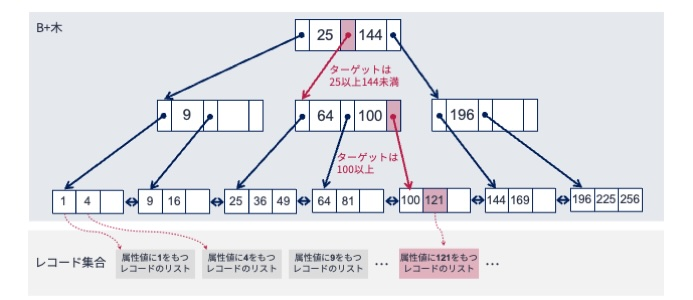
\includegraphics[width=1.0\textwidth]{figure/indexing/b+tree-search.jpg}
    \caption{B+木を用いたレコード探索のイメージ}
    \label{fig:b+tree-search}
\end{figure}

まず，根ノードにアクセスし格納された探索キーを調べます．
探索キーは\graybox{25}と\graybox{144}です．
ターゲットとなる値は\graybox{121}であり，\graybox{25}よりも大きく\graybox{144}よりも小さいです．
よって，探索キー\graybox{25}と\graybox{144}の間にあるポインタをたどります．
ポインタをたどった先にあるノードには，探索キーとして\graybox{64}と\graybox{100}が格納されています．
先ほどと同様，ターゲットとなる値と探索キーの関係を調べると，ターゲット値である\graybox{121}は\graybox{100}より大きいです．
よって，探索キー\graybox{100}の右隣にあるポインタをたどります．
その結果，葉ノードにたどり着きます．
葉ノードに格納された索引キーを左から右に探索すると，左から2番目にターゲット値である索引キー\graybox{121}が見つかります．
所望の索引キーが見つかったので，索引キーからリンクされたレコードを取得します．
これにて探索完了です．

B+木の特徴6に記した条件により，根を除くどの中間ノードも子ノードを少なくとも$d+1$個持つことが保証されています．
これにより，索引キーの総数が$N$の場合，B+木の根ノードから葉ノードへのパスの長さ（木の高さ）は高々$O(\log_{d+1} N)$となります．
各ノード内には最大$2d$個の探索キーがあり，これらをチェックする手間はかかります．
しかし，データベースの探索において真に時間がかかるのは「ディスクからノードをメモリに読み込む処理（ディスクI/O）」です．
B+木を用いた探索では，この非常に重いディスク読み取りの回数がパスの長さと同じ$O(\log_{d+1} N)$回で済むため，膨大なデータに対しても極めて高速な探索が保証されるのです．


\subsection{範囲探索}
B+木を使えば，範囲探索も容易に行えます．
先ほどの例で使ったB+木を使って，属性値がある範囲にあるレコードを探索する手順を示しましょう．

今，属性値が\graybox{10}以上\graybox{40}未満であるレコードをすべて取得したいとします．
手順は以下の通りです（図\ref{fig:range-search}も参照すること）．
\begin{figure}[tb]
    \centering
    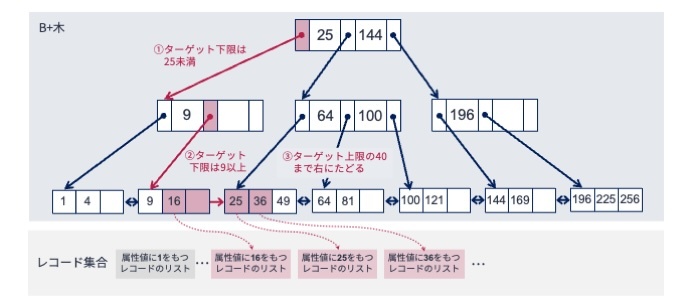
\includegraphics[width=1.0\textwidth]{figure/indexing/range-search.jpg}
    \caption{B+木を用いた範囲探索のイメージ}
    \label{fig:range-search}
\end{figure}

探索条件の下限である\graybox{10}に着目します．
まず根ノードにアクセスし，格納された探索キーを調べます．
探索キーは\graybox{25}と\graybox{144}です．
ターゲットとなる値は\graybox{10}であり，\graybox{25}よりも小さいです．
よって，探索キー\graybox{25}の左にあるポインタをたどります．
ポインタをたどった先にあるノードには，探索キーとして\graybox{9}が格納されています．
ターゲット値は\graybox{10}であるため，探索キー\graybox{9}の右隣にあるポインタをたどります．
その結果，葉ノードにたどり着きます．

葉ノードに格納された索引キーを左から探索すると，左から2番目にターゲット値である\graybox{10}より大きい索引キー\graybox{16}が見つかります．
ところで，ターゲットとなる属性値の上限は\graybox{40}でした．
そこで，先ほど見つけた索引キー\graybox{16}から右側にリンクをたどりながら索引キーが\graybox{40}未満のものをすべて拾い上げていきます．
すると，索引キーとして\graybox{16，25，36}が見つかります．
条件を満たす索引キーがすべて見つかったので，各索引キーからリンクされたレコードを取得します．
これにて範囲探索完了です．


\subsection{B+木の構築・更新}
すでに述べたように，データベースではレコードの追加や更新が度々行われます．
そのため，データベースの更新に応じて索引の更新も必要となります．

B+木は根ノードから葉ノードへのパスの長さが均一になるよう（木の高さのバランスを崩さない）よう，索引を更新するアルゴリズムが提案されています．
直感的には，
\begin{itemize}
\item 新たな索引キーを挿入する場合には，木の構造を崩して木を上に向かって伸ばす
\item 索引キーを削除する場合には，キーの挿入操作の逆を行う
\end{itemize}
といった戦略でB+木を更新します．
B+木の更新アルゴリズムの詳細については「IT Text データベースの基礎\cite{吉川本}」「データベースシステム（改訂2版）\cite{北川本}」「リレーショナルデータベース入門（第3版）\cite{増永本}」などの良書を参照してください．


\section{ハッシュ索引}
B+木のような木構造の索引では，根ノードから葉ノードにまでたどることで，条件にマッチする属性値をもつレコードが格納されている場所を調べます．
探索を容易にするためにB+木では索引を木構造にする工夫をこらしていますが，$O(\log_m{N})$の計算時間をかけて根から葉に向かって木をたどらなければなりません．

仮に，ある値が指定されたときにそれを属性値としてもつレコードの格納位置を「直接」知ることができれば，B+木よりももっとカンタンに求めるレコードを取得することができます．
これを実現するのが，\strong{ハッシュ索引（hash index）} です\cite{Fagin1979, Litwin1980}．
B+木と同様，ハッシュ索引も探索対象となる属性を指定して索引を構築します．

B+木と異なるのは，ハッシュ索引では索引キーの値とレコード（の格納場所）との対応付けを行うために\strong{ハッシュ関数（hash function）} を用いる点です．
ハッシュ関数とは，任意の値を別の都合の良い値（ハッシュ値）に変換するための関数です．
良いハッシュ関数は値の変換にかかる計算コストが低くなるよう設計されています．

$mod_d(x)$は，整数$x$を整数$d$で割ったときの剰余（いわゆる余り）を計算する関数です．
ただし$q$は整数とします．
\begin{equation*}
mod_d(x) = r  \quad \text{where} \,\, x = q \cdot d + r
\end{equation*}
剰余演算は高速に実行できることが知られており，ハッシュ索引を構築するためのハッシュ関数としてしばしば使われます．
例えば，学生情報を格納するテーブル\graybox{学生}に対して，属性\graybox{学籍番号}の値を探索キーとするハッシュ索引を構築するとしましょう．
一般に学籍番号は数字以外の文字も含まれる文字列ですが，計算機の中では文字列も整数値で表現されているので，剰余を計算することは可能です．
そこで，図\ref{fig:hash-index}のように\graybox{学生}テーブルの各レコードの\graybox{学籍番号}の値に剰余を計算する関数を適用し，得られた剰余値が示す記憶装置の場所にレコードを格納します．
イメージとしては，$d＝100$の場合，「学籍番号の下2桁」だけを見て，レコードをどこの場所にしまうかを決める，ということをします．
このようにハッシュ索引を構築しておけば，レコードを取得したい学生の学籍番号から剰余値を1回計算するだけで，必要となる学生情報が格納されている場所を特定し，レコードを取得することができます．
\begin{figure}[tb]
    \centering
    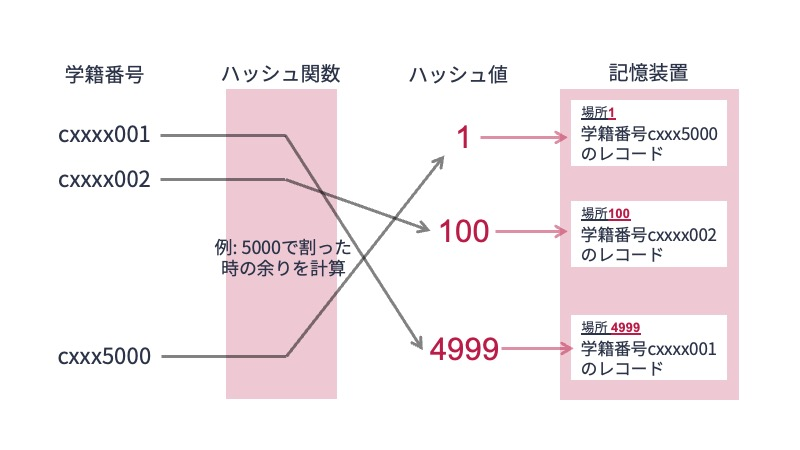
\includegraphics[width=1.0\textwidth]{figure/indexing/hash-index.jpg}
    \caption{ハッシュ索引のイメージ}
    \label{fig:hash-index}
\end{figure}

高速にレコードを取得できるハッシュ索引ですが，致命的な弱点があります．
ハッシュ索引は，各レコードの属性値のハッシュ値に対応するレコードの格納場所を直接割り出しており，探索キーの値が完全一致するものしか見つけられません．
そのため，範囲探索が必要な属性に対しては，B+木のような索引を用いる必要があります．


\section{SQLによる索引の構築}
代表的な索引づけ方法を紹介しましたので，最後に索引を構築するためのSQL文を見ておきましょう．
大抵の関係データベース管理システムでは，コード\ref{code:sql-create-index-structure}のようなSQL文で，テーブルの特定の属性に対して索引を構築することができます（「インデックスを張る」ともいう）．
\begin{figure}[h]
    \begin{minted}[gobble=1,
        bgcolor=background,
        fontsize=\small,
        linenos=false,
        xleftmargin=0em]{sql}

    CREATE INDEX インデックス名
        ON テーブル名 (索引の対象となる属性名)
    USING 索引種別;

    \end{minted}
    \captionsetup{name=コード}
    \caption{索引構築のためのSQLの構文}
    \label{code:sql-create-index-structure}
\end{figure}

例えば\graybox{product}テーブルの属性\graybox{price}に関してB+木を使った索引を構築したい場合は，コード\ref{code:sql-create-btree-index}のようなSQL文を使います．
\begin{figure}[h]
    \begin{minted}[gobble=1,
        bgcolor=background,
        fontsize=\small,
        linenos=false,
        xleftmargin=0em]{sql}

    CREATE INDEX product_price_idx
        ON product (price)
    USING btree;

    \end{minted}
    \captionsetup{name=コード}
    \caption{B+木を使った索引を構築するためのSQL文}
    \label{code:sql-create-btree-index}
\end{figure}

一般に，主キーや外部キーとして指定された属性には自動的に索引が構築されますが，それ以外の属性に索引を構築したい場合は上記のようなSQL文を発行する必要があります．
問い合わせに対する応答速度が遅い場合，索引の構築は非常に効果的です．
一方，索引は記憶領域を余分に消費するので，無闇に索引を構築するのは避けるべきです．



% ---------------------------------------
\section{クイズ}
% ---------------------------------------

\subsection*{Q1. B+木の探索（1/2）}
図\ref{fig:b+tree}に示されたB+木において，属性$A$の値が16であるレコードを探索する際，根ノードから順にたどる探索キー（比較対象となる値）をすべて列挙しなさい．

\subsection*{Q2. B+木の探索（2/2）}
図\ref{fig:b+tree}に示されたB+木において，範囲検索として属性$A$の値が25以上81以下のレコードを取得する場合，葉ノード（最下層）においてスキャンされる索引キーを順番にすべて答えなさい．


\subsection*{Q3. 索引づけの選択}
あるオンラインショッピングサイトのデータベースには，以下の関係スキーマを持つ「注文」テーブルがあります．
「配送ステータス」には「未発送」「発送済」「キャンセル」の3種類の値のいずれかが入ります．
このデータベースでは，主キーである「注文ID」には自動的にB+木で索引づけがなされています．
\begin{equation}
\textbf{注文}(\underline{\text{注文ID}}, \text{ユーザID}, \text{商品ID}, \text{注文日}, \text{配送ステータス})
\end{equation}

システムを運用したところ，特定の条件での検索に時間がかかっていることが判明したため，追加で索引づけすることを検討しています．
以下の候補のうち，新たに索引を構築する対象として最も不適切なものはどれでしょうか．
その理由とともに答えなさい．

\begin{itemize}
\item 注文ID
\item ユーザID（ある特定のユーザの注文履歴を一覧表示する処理が頻繁に実行される）
\item 注文日（ある特定の日付の売り上げを集計する処理が頻繁に実行される）
\item 配送ステータス（まだ発送されていない注文を絞り込む処理が実行される）
\end{itemize}


\subsection*{Q4. 索引づけとトレードオフ}
企業の社員情報を管理する，以下の関係スキーマを持つ「社員」テーブルがあります．
\begin{equation}
\textbf{社員}(\underline{\text{社員ID}}, \text{氏名}, \text{部署名}, \text{入社年度}, \text{給与})
\end{equation}

このデータベースに対して，以下の2種類の問い合わせが非常に高い頻度で実行されることが分かりました．
\begin{itemize}
    \item 特定の部署に所属する社員の一覧を取得する（例: \graybox{WHERE 部署名 = `営業部'}）
    \item 特定の入社年度の社員の一覧を取得する（例: \graybox{WHERE 入社年度 = 2020}）
\end{itemize}
一方で，この会社では毎月多くの新入社員や中途社員が入社するため，「社員」テーブルに対するレコードの追加も頻繁に行われます．

属性「部署名」と「入社年度」のそれぞれに索引づけを行うべきでしょうか．
索引を構築することによるメリット（検索速度の向上）とデメリット（更新コストの増加など）のトレードオフを踏まえ，あなたの考えを説明しなさい．
